\documentclass[11pt,a4paper]{article}
\usepackage[utf8]{inputenc}
\usepackage[T1]{fontenc}
\usepackage[margin=1in]{geometry}
\usepackage{hyperref}
\usepackage{xcolor}
\usepackage{float}
\usepackage{listings}
\usepackage{upquote}
\usepackage{amsmath}

\lstset{
    basicstyle=\ttfamily\small,
    breaklines=true,
    breakatwhitespace=false,
    frame=single,
    numbers=left,
    numberstyle=\tiny,
    backgroundcolor=\color{gray!10},
    keywordstyle=\color{blue},
    commentstyle=\color{green!50!black},
    stringstyle=\color{red},
    showstringspaces=false
}

\title{\textbf{Practice 2 -- Stretch Robot Kinematics}}
\author{
    Robotics and Cyber-Physical Systems \\
    School of Sciences and Engineering \\
    Tecnol\'ogico de Monterrey
}
\date{}

\begin{document}

\maketitle

\section*{Introduction}

In this practice, you will control the Stretch robot using two complementary
interfaces. First, you will use the robot's standard Python API to command exact
joint positions. You will then use the \texttt{stretch\_tools} package to send
normalized velocity commands and combine autonomous motion with manual input.

The same scripts can run in the MuJoCo simulator and on the physical robot. The
simulator package implements the most important parts of the physical Stretch
API, allowing the backend to be selected with a simple import fallback.

The practice has three parts:

\begin{enumerate}
    \item Move the robot through a fixed grasping sequence using position commands.
    \item Drive one joint with a sine-wave velocity while reading its position.
    \item Add full keyboard and gamepad override to the sine-wave behavior.
\end{enumerate}

\subsection*{Before You Begin}

Update the repository and synchronize its dependencies before starting. Back up
any uncommitted work before using commands that overwrite local changes.

\begin{lstlisting}[language=bash]
git pull
uv sync
\end{lstlisting}

Always enable collision management before moving the physical robot:

\begin{lstlisting}[language=Python]
stretch.enable_collision_mgmt()
\end{lstlisting}

Make sure the robot and its surroundings have enough clearance before running
any program. Keep the emergency stop accessible when working with the physical
robot.

\section{Part 1: Position Commands with the Robot API}

The standard Stretch API begins with a \texttt{Robot} object. Use the following
import pattern so the same file selects the physical API when it is installed and
falls back to the simulator otherwise:

\begin{lstlisting}[language=Python]
try:
    import stretch_body.robot as robot
except ImportError:
    import stretch_mujoco_api.robot as robot
\end{lstlisting}

Create, start, and safely stop the robot as follows:

\begin{lstlisting}[language=Python]
if __name__ == "__main__":
    stretch = robot.Robot()
    stretch.startup()
    stretch.enable_collision_mgmt()

    try:
        # Robot commands go here.
        pass
    finally:
        stretch.stop()
\end{lstlisting}

The \texttt{finally} block runs even if the program encounters an error or the
user presses Ctrl+C. It ensures that the robot connection and simulator process
are closed cleanly.

\subsection*{Accessing the joints}

The lift and arm are available directly from the robot:

\begin{lstlisting}[language=Python]
lift = stretch.lift
arm = stretch.arm
\end{lstlisting}

Head and end-of-arm joints are retrieved by name:

\begin{lstlisting}[language=Python]
head_pan = stretch.head.get_joint("head_pan")
head_tilt = stretch.head.get_joint("head_tilt")

wrist_pitch = stretch.end_of_arm.get_joint("wrist_pitch")
wrist_roll = stretch.end_of_arm.get_joint("wrist_roll")
wrist_yaw = stretch.end_of_arm.get_joint("wrist_yaw")
gripper = stretch.end_of_arm.get_joint("stretch_gripper")
\end{lstlisting}

\subsection*{Movement commands}

The principal joint methods are:

\begin{center}
\begin{tabular}{|l|l|}
\hline
\textbf{Method} & \textbf{Behavior} \\
\hline
\texttt{move\_to(position)} & Move to an absolute position \\
\texttt{move\_by(distance)} & Move relative to the current position \\
\texttt{set\_velocity(velocity)} & Move continuously at the requested velocity \\
\hline
\end{tabular}
\end{center}

Lift and arm positions are measured in meters. Head and wrist positions are
measured in radians. The gripper uses percentage-like commands, normally in the
range $[-100,100]$, where positive values open the gripper and negative values
close it farther.

A position command follows this pattern:

\begin{lstlisting}[language=Python]
stretch.lift.move_to(0.5)
stretch.push_command()
stretch.wait_command()
\end{lstlisting}

\texttt{push\_command()} sends queued commands to the robot.
\texttt{wait\_command()} blocks until the commanded motion is complete. Always
push each movement before waiting for it. Waiting after every step is especially
important when the order of operations prevents collisions.

Joint state is available through the \texttt{status} dictionary:

\begin{lstlisting}[language=Python]
position = stretch.lift.status["pos"]
velocity = stretch.lift.status["vel"]
print(position, velocity)
\end{lstlisting}

The complete robot state can be retrieved with \texttt{stretch.get\_status()}.

\subsection*{Activity: Create \texttt{p2\_1\_grab.py}}

Create a new Python file named \texttt{p2\_1\_grab.py} from scratch. Do not copy a
completed solution. Include the cross-environment import, robot startup,
collision management, and a \texttt{try}/\texttt{finally} cleanup block.

Inside the \texttt{try} block, command the following sequence in this exact order:

\begin{enumerate}
    \item Move the lift to $0.41\,\text{m}$.
    \item Open the gripper to $50$.
    \item Extend the arm to $0.14\,\text{m}$.
    \item Close the gripper toward $0.5$.
    \item Raise the lift to $0.60\,\text{m}$.
\end{enumerate}

Call \texttt{stretch.push\_command()} and \texttt{stretch.wait\_command()} after
every movement. The gripper may stop before reaching $0.5$ because the object
prevents its fingers from fully closing. This is normal and represents a
successful grasp.

Run the program with:

\begin{lstlisting}[language=bash]
uv run p2_1_grab.py
\end{lstlisting}

\textbf{Expected result:} The robot lowers to the object, opens its gripper,
extends its arm, grasps the object, and lifts it. The ordering should prevent the
arm and gripper from colliding with the environment.

\begin{figure}[H]
    \centering
    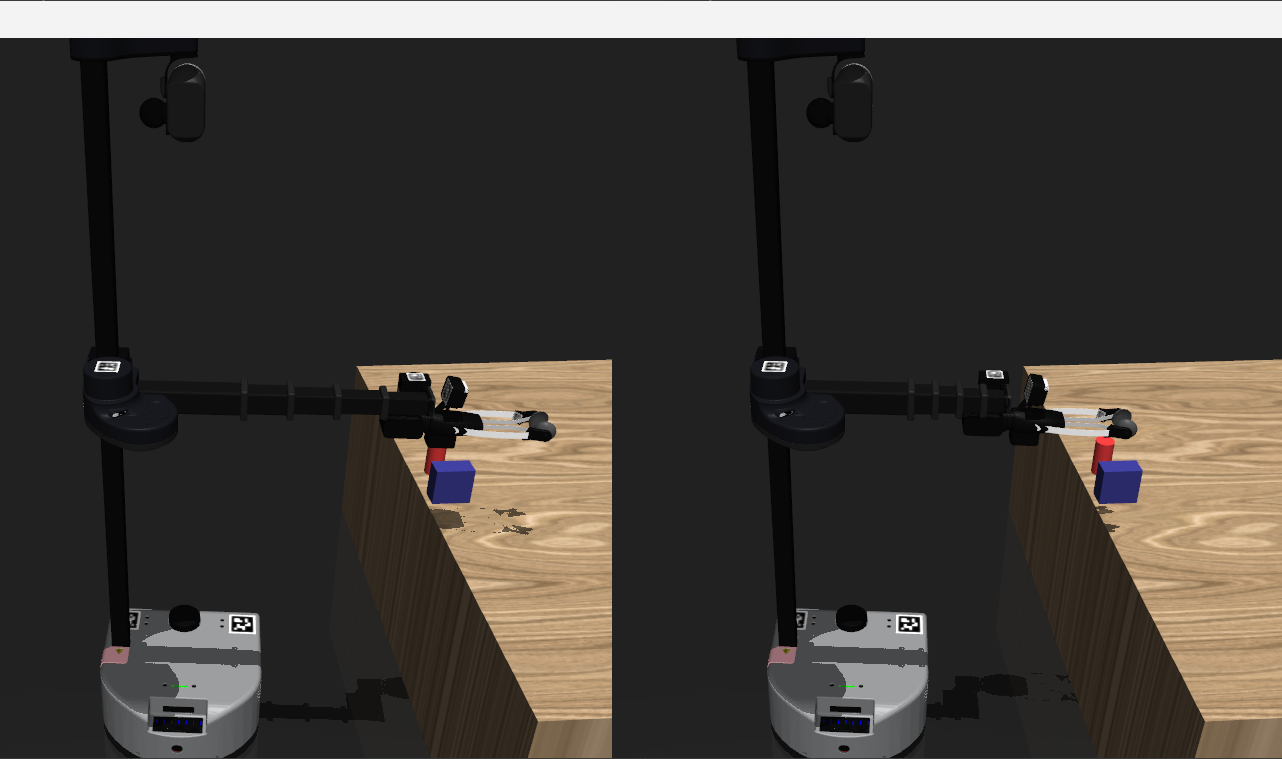
\includegraphics[width=0.6\textwidth]{arm_out.png}
    \caption{The arm extending as part of the grasping sequence.}
    \label{fig:grab-arm-out}
\end{figure}

\section{Part 2: Sinusoidal Velocity Control and Joint State}

Position commands are useful for discrete motions. Continuous behaviors are
often easier to express as normalized joint velocities. The
\texttt{NormVelController} class from \texttt{stretch\_tools} accepts sparse
command dictionaries with values in $[-1,1]$:

\begin{lstlisting}[language=Python]
from stretch_tools import NormVelController

controller = NormVelController(stretch)
controller.set_command({"head_pan_counterclockwise": 0.5})
\end{lstlisting}

A value of $1$ requests the configured maximum speed in the positive named
direction. A value of $-1$ requests maximum speed in the opposite direction.
A value of $0$ stops and holds that joint.

Command dictionaries are sparse. If a key is omitted, the controller does not
send any command to that joint. This allows omitted joints to continue following
commands issued through the standard robot API.

The available normalized command keys are:

\begin{center}
\begin{tabular}{|l|l|}
\hline
\textbf{Key} & \textbf{Positive direction} \\
\hline
\texttt{base\_forward} & Base translates forward \\
\texttt{base\_counterclockwise} & Base rotates left \\
\texttt{lift\_up} & Lift moves upward \\
\texttt{arm\_out} & Arm extends \\
\texttt{wrist\_roll\_counterclockwise} & Wrist rolls left \\
\texttt{wrist\_pitch\_up} & Wrist pitches upward \\
\texttt{wrist\_yaw\_counterclockwise} & Wrist yaws left \\
\texttt{head\_pan\_counterclockwise} & Head pans left \\
\texttt{head\_tilt\_up} & Head tilts upward \\
\texttt{gripper\_open} & Gripper opens \\
\hline
\end{tabular}
\end{center}

\subsection*{Activity: Create \texttt{p2\_2\_sine.py}}

Create a new script named \texttt{p2\_2\_sine.py}. Set up the robot using the
same import and lifecycle pattern from Part 1, then instantiate a
\texttt{NormVelController}.

Make the head pan continuously using the normalized velocity:

\[
v(t)=\sin(\omega t), \qquad \omega=2.0
\]

Use \texttt{time.monotonic()} to measure elapsed time:

\begin{lstlisting}[language=Python]
started = time.monotonic()

while True:
    elapsed = time.monotonic() - started
    velocity = math.sin(2.0 * elapsed)
\end{lstlisting}

On every iteration:

\begin{enumerate}
    \item Calculate the sinusoidal velocity.
    \item Send it using the \texttt{head\_pan\_counterclockwise} command key.
    \item Read the head-pan position from
    \texttt{stretch.head.get\_joint("head\_pan").status["pos"]}.
    \item Print the velocity and position.
    \item Sleep for $0.1$ seconds before the next update.
\end{enumerate}

Your loop should contain the following core operations:

\begin{lstlisting}[language=Python]
command = {"head_pan_counterclockwise": velocity}
controller.set_command(command)

position = head_pan.status["pos"]
print(f"velocity={velocity:.3f}, position={position:.3f}")
time.sleep(0.1)
\end{lstlisting}

Run the program with:

\begin{lstlisting}[language=bash]
uv run p2_2_sine.py
\end{lstlisting}

\textbf{Expected result:} The head pans smoothly left and right. The terminal
prints a sinusoidal normalized velocity and the corresponding head angle in
radians.

\begin{figure}[H]
    \centering
    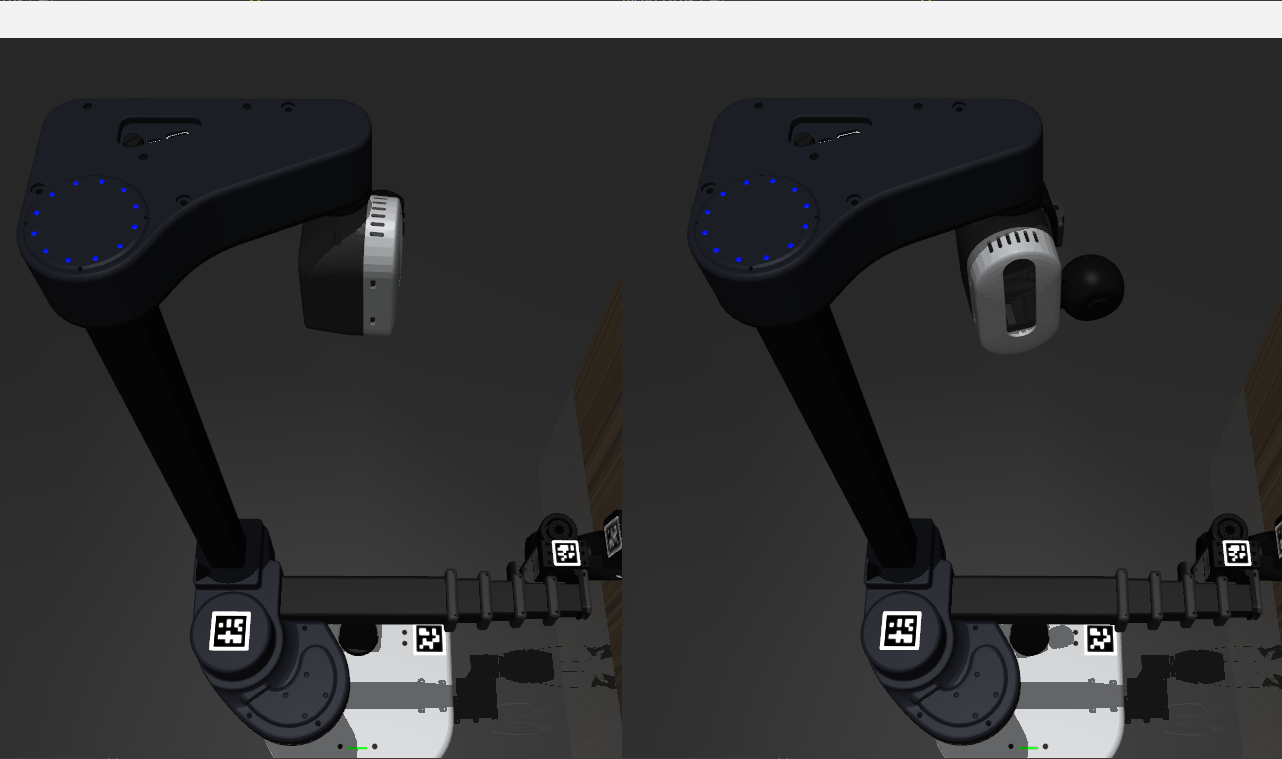
\includegraphics[width=0.6\textwidth]{head_pan.png}
    \caption{Head-pan motion produced by a sinusoidal velocity command.}
    \label{fig:sine-head-pan}
\end{figure}

\section{Part 3: Manual Override}

Autonomous and manual commands can be combined through
\texttt{TeleopProvider}. It reads the configured keyboard and gamepad inputs and
uses proportional blending to override an algorithmic command only where the
operator provides input.

Import and create it as follows:

\begin{lstlisting}[language=Python]
from stretch_tools import NormVelController, TeleopProvider

controller = NormVelController(stretch)
teleop = TeleopProvider(robot=stretch)
\end{lstlisting}

Given an autonomous command dictionary, obtain the final command with:

\begin{lstlisting}[language=Python]
command = teleop.get_manual_override(command_autonomous)
controller.set_command(command)
\end{lstlisting}

In the default autonomous mode, idle teleop inputs leave the autonomous command
unchanged. Moving a stick or holding a mapped key proportionally overrides the
affected joint. Full input takes complete control of that joint.

Press the Y face button or the \texttt{y} key to toggle manual mode. In manual
mode, the autonomous dictionary is ignored and only teleop commands are sent.
Press it again to restore autonomous motion with proportional override.

Useful keyboard controls include:

\begin{center}
\begin{tabular}{|l|l|}
\hline
\textbf{Keys} & \textbf{Control} \\
\hline
W/S & Base forward/backward \\
A/D & Base rotation \\
Z/X & Lift \\
V/C & Arm \\
M/N & Gripper \\
J/L & Wrist yaw \\
O/U & Wrist roll \\
I/K & Wrist pitch \\
H & Toggle D-pad control between wrist and head \\
F & Hold for fast base mode when the lift is below $0.34\,\text{m}$ \\
P & Hold for precision mode \\
Y & Toggle autonomous/manual mode \\
\hline
\end{tabular}
\end{center}

The left trigger proportionally slows all joints, reaching $10\%$ speed when
fully pressed. The right trigger proportionally increases base speed from the
default safe limit to full speed, but only while the lift is below
$0.34\,\text{m}$.

\subsection*{Activity: Create \texttt{p2\_3\_manual\_override.py}}

Copy your completed Part 2 program:

\begin{lstlisting}[language=bash]
cp p2_2_sine.py p2_3_manual_override.py
\end{lstlisting}

Then:

\begin{enumerate}
    \item Import \texttt{TeleopProvider} from \texttt{stretch\_tools}.
    \item Create a provider with \texttt{TeleopProvider(robot=stretch)}.
    \item Keep calculating the same sinusoidal autonomous command.
    \item Pass that dictionary to \texttt{teleop.get\_manual\_override()}.
    \item Send the returned dictionary through \texttt{controller.set\_command()}.
    \item Continue printing head-pan velocity and position.
\end{enumerate}

The central loop should now follow this pattern:

\begin{lstlisting}[language=Python]
command_autonomous = {
    "head_pan_counterclockwise": velocity,
}
command = teleop.get_manual_override(command_autonomous)
controller.set_command(command)
\end{lstlisting}

Run the program with:

\begin{lstlisting}[language=bash]
uv run p2_3_manual_override.py
\end{lstlisting}

\textbf{Expected result:}

\begin{itemize}
    \item With no input, the head continues following the sine wave.
    \item Manual input can proportionally override any mapped joint.
    \item In manual mode, the sinusoidal command is disabled.
    \item Returning to autonomous mode resumes the sine-wave behavior.
\end{itemize}

\begin{figure}[H]
    \centering
    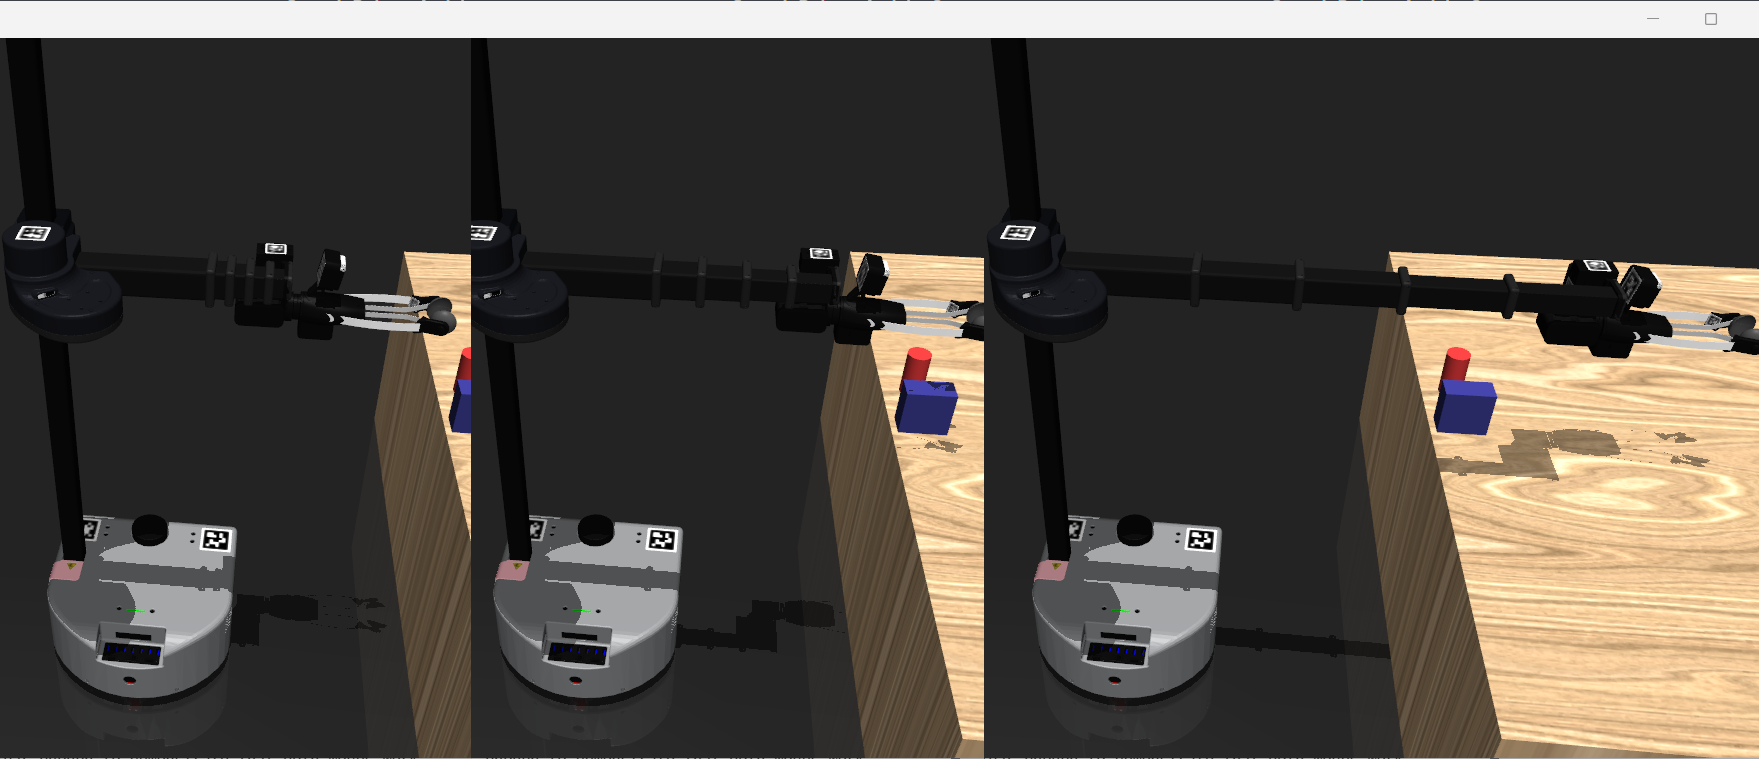
\includegraphics[width=0.6\textwidth]{arm_out_override.png}
    \caption{An example of manual input overriding an autonomous joint command.}
    \label{fig:manual-override}
\end{figure}

\section*{Deliverable}

Submit the three Python files and a concise video demonstrating:

\begin{enumerate}
    \item The ordered grasp-and-lift sequence from \texttt{p2\_1\_grab.py}.
    \item Sinusoidal head motion and live position output from
    \texttt{p2\_2\_sine.py}.
    \item Autonomous sine-wave motion, proportional manual override, manual-mode
    toggling, and return to autonomous mode in
    \texttt{p2\_3\_manual\_override.py}.
\end{enumerate}

The video should clearly show that each behavior works. Keep it concise; between
one and two minutes is sufficient.

\end{document}
